\title{palsr: Projecting the Locations of Moving Actors for Spatial Models of
Dyadic Interaction}
\author{by Sangyeon Kim, Howard Liu, and Bruce A. Desmarais}

\maketitle

\abstract{%
Many actors studied in the social sciences---armed groups, firms, diplomats,
migrating populations---have no fixed geographic location, and the place at which
two such actors interact is itself a meaningful outcome. Standard spatial tools
assume actors sit at fixed points and therefore cannot be applied directly. The
\pkg{palsr} package implements the Projected Actor Location (PALS) method of
\citet{kim2023pals}, which uses exponential-smoothing weights over the
spatiotemporal histories of a focal actor and its interaction partners to project
where a mobile actor effectively ``is'' at any moment, and tunes those weights to
predict the locations of future interactions. The package provides a validated
event-data container, maximum-similarity parameter estimation by minimizing
great-circle prediction error, projection of actor locations at arbitrary times,
construction of the dyadic distance covariates used in downstream interaction
models, and nonparametric bootstrap uncertainty with Rubin's Rules pooling.
Performance-critical kernels are implemented in C++ via \CRANpkg{Rcpp}. We
illustrate the full workflow on a bundled dataset of armed-conflict events in
Nigeria.
}

\section{Introduction}

A great deal of social-scientific inquiry is \emph{dyadic}: the unit of analysis
is a pair of actors, and a central question is whether, how, and where the two
interact. In the study of geopolitical relations---alliances, conflict,
cooperation, trade---one of the most robust predictors of interaction is the
geographic distance between the actors involved \citep{gleditsch2001, ward2007}.
When the actors are states with fixed capitals or centroids, this distance is
trivial to compute and treat as an exogenous covariate.

A large and growing share of substantively important actors, however, are not
fixed in space. Rebel groups, militias, terrorist organizations, peacekeeping
deployments, and non-governmental organizations move through a theatre of
operations over time, and the fine-grained, geocoded event data that now document
them---such as the Armed Conflict Location and Event Data project
\citep[ACLED;][]{acled}---record \emph{where each interaction happened} but assign
the actors themselves no persistent coordinates. Treating these actors as
fixed-location entities discards exactly the spatial dynamics that drive their
interactions.

Existing spatial software for R does not fill this gap. General geospatial
toolkits such as \CRANpkg{sf} \citep{sf} and spatial point-process libraries such
as \CRANpkg{spatstat} \citep{spatstat} are powerful, but they operate on objects
with given coordinates; they provide no way to \emph{infer} a moving actor's
effective location, let alone one tuned to predict future interactions.
Conversely, the dyadic interaction models common in political science and
economics take inter-actor distance as an input. \citet{kim2023pals} introduced
the Projected Actor Location (PALS) method to bridge this gap, and showed that
PALS-based distances substantially improve the prediction of subnational conflict
relative to naive location measures. That article, however, was accompanied only
by replication scripts specific to a single application.

This paper introduces \CRANpkg{palsr}, an R package that turns PALS into reusable,
documented, and tested research software. The package lets applied researchers
apply PALS to their own dyadic event data without re-deriving the estimator,
construct the distance covariates needed by downstream interaction models, and
propagate estimation uncertainty into those models through a principled bootstrap.
After reviewing the method, we describe the package's design and walk through a
complete analysis of armed-conflict events in Nigeria.

\section{The PALS method}

\subsection{Projecting a location}

PALS represents the location of a mobile actor at a prediction time as a
recency-weighted average of the locations of events in which the actor, and its
past interaction partners, were involved. Let $i$ be a \emph{focal} actor and $t$
a prediction time. Write $e$ for an event with location $g(e)$ (a
longitude--latitude pair) and age $t - t(e)$ at time $t$. PALS uses only events
that occurred strictly before $t$.

The projected location is a convex combination of two components. The
\emph{focal} component is a recency-weighted mean of the locations of $i$'s own
past events; the \emph{alter} component is a recency-weighted mean of the
locations of events involving the actors that $i$ has interacted with (its
\emph{alters}). Formally,
%
\begin{equation}
  g_i(t) = (1-\pi)\sum_{e \in E_i} W_i(e)\, g(e)
         \;+\; \pi \sum_{e \in E_k} W_k(e)\, g(e),
  \qquad
  \pi = \mathrm{logistic}(\gamma + \eta\, v),
  \label{eq:pals}
\end{equation}
%
where $E_i$ and $E_k$ are the focal and alter event sets. The weights decay with
event age in the manner of exponential smoothing \citep{gardner2006},
%
\begin{equation}
  W_i(e) \propto \bigl(\text{age}(e)^{\alpha} + \epsilon\bigr)^{-1},
  \qquad
  W_k(e) \propto \bigl(\text{age}(e)^{\beta} + \epsilon\bigr)^{-1},
\end{equation}
%
normalized to sum to one within each component, with a small offset $\epsilon$ to
keep contemporaneous events finite. The mixing weight $\pi$ governs how much the
projection leans on the alters rather than the focal actor's own history. It
depends through an intercept $\gamma$ and a slope $\eta$ on a statistic $v$ that
compares the number of focal events $n_i$ with the number of alter events $n_k$,
$v = (n_i / n_k)^{1/\sqrt{n_k}}$, so that an actor with a sparse personal history
but active partners can borrow location information from those partners.

The method therefore has four parameters: $\alpha$ (decay of the focal history),
$\beta$ (decay of the alter histories), and $\gamma$ and $\eta$ (the focal-versus-
alter mixing weight). A reduced \emph{one-parameter} model fixes $\pi = 0$, using
only the focal history and estimating $\alpha$ alone; it is fast and, as we show
below, frequently competitive.

\subsection{Estimating the parameters}

The parameters are chosen to maximize the spatial similarity between predicted and
observed interaction locations. The predicted location of an interaction between
two actors is the mean of their two projected locations, and prediction proceeds
by ``marching forward'' through time: each observed event is predicted using only
events strictly preceding it. The objective is the mean great-circle (Haversine)
distance between predicted and observed locations,
%
\begin{equation}
  Q(\theta) = \frac{1}{n}\sum_{e} d_{\mathrm{H}}\!\bigl(g(e),\,
              \hat g(e;\theta)\bigr),
\end{equation}
%
minimized over the parameter vector $\theta$ with \code{stats::optim} (Brent's
method for the one-parameter model, Nelder--Mead for the full model). Because the
projection is recomputed for every event at every candidate $\theta$, estimation
re-projects every actor across a grid of times many times over; the inner
projection and distance kernels are implemented in C++ for speed (see below).

\section{The palsr package}

\subsection{Event data}

The central data object is a \code{pal\_events} table, a validated
\code{data.frame} subclass with one row per dyadic event and canonical columns
\code{actor1}, \code{actor2}, \code{time} (a \code{Date}), \code{lon}, and
\code{lat}. The constructor \code{pal\_events()} maps arbitrary column names onto
this schema, coerces types, checks coordinate ranges, drops incomplete or
self-dyadic rows, and sorts by time:

\begin{verbatim}
library(palsr)
raw <- data.frame(from = c("A", "A", "B"), to = c("B", "C", "C"),
                  when = as.Date(c("2001-01-01", "2001-06-01", "2002-01-01")),
                  x = c(7.1, 8.0, 7.5), y = c(9.0, 9.4, 10.1))
ev <- pal_events(raw, actor1 = "from", actor2 = "to",
                 time = "when", lon = "x", lat = "y")
\end{verbatim}

\subsection{Main functions}

The package exposes the PALS workflow through a small set of functions, summarized
in Table~\ref{tab:functions}.

\begin{table}[t]
\centering
\begin{tabular}{ll}
\toprule
Function & Purpose \\
\midrule
\code{pal\_events()} & Build and validate a dyadic event table \\
\code{pals\_params()} & Specify a parameter set directly \\
\code{estimate\_pals()} & Estimate parameters by Haversine-error minimization \\
\code{project\_pal()}, \code{project\_pals()} & Project actor locations at given times \\
\code{predict\_event\_locations()} & Predict dyadic interaction locations \\
\code{pal\_distance()} & Dyadic distance between projected locations \\
\code{bootstrap\_pals()} & Nonparametric bootstrap uncertainty \\
\code{pool\_rubin()} & Pool replicate estimates with Rubin's Rules \\
\code{simulate\_conflict\_events()} & Simulate mobile-actor interaction data \\
\bottomrule
\end{tabular}
\caption{The main user-facing functions of \pkg{palsr}.}
\label{tab:functions}
\end{table}

A model is fit with \code{estimate\_pals()}, which returns an object of class
\code{pals\_fit} with \code{print}, \code{summary}, \code{coef}, and \code{predict}
methods. Given a fit (or a hand-specified \code{pals\_params} object),
\code{project\_pals()} returns the projected location of each actor at one or more
times, \code{predict\_event\_locations()} predicts interaction locations and scores
them against observed coordinates, and \code{pal\_distance()} constructs the dyadic
distance covariate---optionally log-transformed---that enters downstream models of
who interacts with whom.

\subsection{Implementation}

The projection kernel and the great-circle distance are implemented in C++ and
exposed through \CRANpkg{Rcpp}. A batched kernel evaluates the projection for all
events of an estimation problem in a single compiled call, so that each evaluation
of the objective during optimization avoids the overhead of repeated R-level
iteration. The pure-R reference implementation of the kernel is retained and is
checked against the compiled version in the package's test suite, which uses
\CRANpkg{testthat}.

\subsection{Bundled data}

So that the full workflow can be learned and reproduced without external data, the
package bundles two datasets. \code{nigeria\_acled} contains 1,549 dyadic conflict
events among 37 actors in Nigeria between 1997 and 2016, drawn from the public
replication archive for \citet{kim2023pals}; the underlying event records come
from ACLED. \code{nigeria\_sim} is a deterministic, seeded simulation produced by
\code{simulate\_conflict\_events()}, which generates events among actors that drift
slowly through space and interact preferentially with nearby partners.

\section{Illustration}

We illustrate \pkg{palsr} with the bundled \code{nigeria\_acled} data. We first fit
the one-parameter model, which estimates only the focal decay $\alpha$:

\begin{verbatim}
data(nigeria_acled)
fit1 <- estimate_pals(nigeria_acled, model = "one")
coef(fit1)
#>    alpha
#> 1.240806
\end{verbatim}

The fitted $\alpha \approx 1.24$ implies steeply decaying weights, so a projected
location is dominated by an actor's most recent events. At the optimum the mean
prediction error is about 147~km over the 1,540 events with usable history. The
full four-parameter model adds the alter component:

\begin{verbatim}
fit4 <- estimate_pals(nigeria_acled, model = "four")
coef(fit4)
#>       alpha        beta       gamma         eta
#>  1.24058   0.01258   -11.32243    -9.70853
\end{verbatim}

Here the large negative $\gamma$ drives the mixing weight $\pi$ to essentially
zero, so the four-parameter fit reproduces the one-parameter fit almost exactly
(an objective of 147~km in both cases). This recovers a substantive finding of
\citet{kim2023pals}: in this application an actor's own recent history is far more
informative about where it will next be engaged than the histories of its
partners, and the parsimonious one-parameter model loses little.

Because the projection is recomputed as time advances, each actor traces a
\emph{trajectory} through space. Figure~\ref{fig:traj} shows the projected paths of
four actors at yearly intervals, drawn over the cloud of observed events:

\begin{verbatim}
actors <- c("Boko Haram", "Fulani Ethnic Militia (Nigeria)",
            "Ijaw Ethnic Militia (Nigeria)")
dates  <- as.Date(sprintf("%d-01-01", 2005:2016))
traj   <- project_pals(nigeria_acled, actors = actors,
                       predict_time = dates, params = fit1)
\end{verbatim}

\begin{figure}[t]
\centering
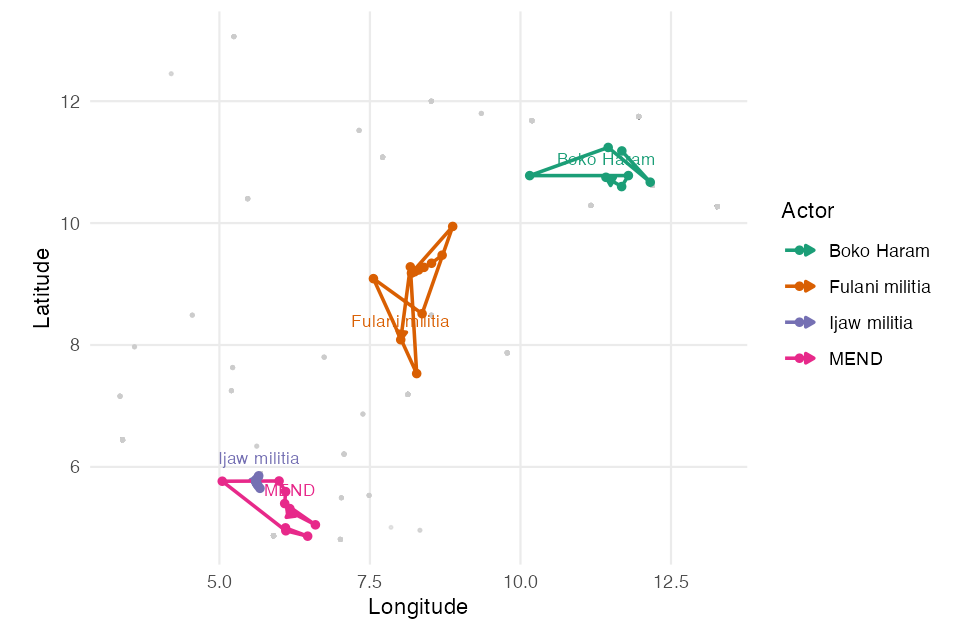
\includegraphics[width=0.85\textwidth]{figure-trajectories.png}
\caption{PALS-projected trajectories of four actors in the \code{nigeria\_acled}
data, fit with the one-parameter model and projected at yearly intervals from 2005
to 2016. Grey points are the observed dyadic events; coloured paths trace each
actor's projected location over time, with arrows pointing forward in time. The
projections separate the actors into distinct, drifting regions of operation.}
\label{fig:traj}
\end{figure}

The projected locations feed directly into models of dyadic interaction. The
function \code{pal\_distance()} returns the great-circle distance between two
actors' projected locations at a given time, the key spatial covariate of
\citet{kim2023pals}:

\begin{verbatim}
dyads <- data.frame(actor1 = "Boko Haram",
                    actor2 = "Fulani Ethnic Militia (Nigeria)",
                    time   = as.Date("2014-06-01"))
pal_distance(nigeria_acled, dyads, fit1, transform = "log")
#>      actor1                          actor2       time pal_distance pal_log_distance
#>  Boko Haram Fulani Ethnic Militia (Nig) 2014-06-01        445.6            6.099
\end{verbatim}

\subsection{Quantifying uncertainty}

Parameter and projection uncertainty are quantified by a nonparametric bootstrap.
\code{bootstrap\_pals()} resamples events with replacement, re-estimates the model
on each replicate, and returns bootstrap standard errors and percentile intervals:

\begin{verbatim}
bt <- bootstrap_pals(nigeria_acled, R = 20, model = "one", seed = 1)
summary(bt)
#>   term estimate boot_mean boot_se lower upper
#>  alpha    1.241      1.240   0.100 1.075 1.451
\end{verbatim}

The 95\% percentile interval for $\alpha$ is roughly $[1.08, 1.45]$, comfortably
away from zero. When a downstream estimand---for example a regression coefficient
in a model of conflict that uses PAL distances---is computed on each replicate, the
replicates can be treated as multiple imputations and combined with Rubin's Rules
\citep{rubin1987} using \code{pool\_rubin()}, which propagates both within- and
between-replicate uncertainty and optionally reports Barnard--Rubin degrees of
freedom.

\section{Summary}

\pkg{palsr} provides a complete, tested implementation of the Projected Actor
Location method for analysts who study interactions among geographically mobile
actors. It turns a method that previously existed only as application-specific
replication code into general-purpose software: validated data structures,
maximum-similarity estimation with compiled kernels, projection and dyadic-distance
construction, and bootstrap-based uncertainty quantification, together with bundled
data and a vignette so the workflow can be reproduced end to end. The package is
available from CRAN at \url{https://CRAN.R-project.org/package=palsr} and is
developed openly at \url{https://github.com/bdesmarais/palsr}; its replication
archive and the underlying method are documented in \citet{kim2023pals}.

\section{Acknowledgements}

This material is based upon work supported by the U.S. National Science Foundation.
The development of PALS and this software was supported by the collaborative
project ``Georelational Dynamics in Collective Action'' (awards 2446647 and
2446646), with additional support to B.A.D.\ from awards 2449569 and 2318460. We
thank the developers of \CRANpkg{Rcpp} for the tooling that underpins the
package's performance.

\bibliography{palsr}

\address{Sangyeon Kim\\
Division of Communication and Media, Ewha Womans University\\
Seoul, Republic of Korea\\
\textit{ORCID: \href{https://orcid.org/0000-0001-9105-8598}{0000-0001-9105-8598}}}

\address{Howard Liu\\
Department of Political Science, University of South Carolina\\
Columbia, SC, USA\\
\textit{ORCID: \href{https://orcid.org/0000-0002-3479-9864}{0000-0002-3479-9864}}}

\address{Bruce A. Desmarais\\
Department of Political Science, Pennsylvania State University\\
University Park, PA, USA\\
\textit{ORCID: \href{https://orcid.org/0000-0002-3031-8883}{0000-0002-3031-8883}}\\
\href{mailto:bdesmarais@psu.edu}{bdesmarais@psu.edu}}
